\documentclass[a4paper,11pt]{article}

%\usepackage[utf8]{inputenc}
\usepackage{graphicx}
\usepackage{url}
\usepackage{float}
\usepackage{times}
\usepackage{multirow}
\usepackage{listings}
\usepackage{times}
\usepackage{paralist}
\usepackage{epsfig}
\usepackage{subfigure}
\usepackage[hypertex]{hyperref}
\usepackage{subfigure}
\usepackage{color}
\usepackage{ifpdf}
\usepackage{wrapfig}

\usepackage{texdraw}
\usepackage{epsf}
\usepackage{array}
\usepackage{cite}
\usepackage{enumitem}
\usepackage{verbatim}
\usepackage{setspace}
\sloppy
\usepackage{geometry}



\newcommand{\I}[1]{\textit{#1}}
\newcommand{\B}[1]{\textbf{#1}}
\newcommand{\BI}[1]{\textbf{\textit{#1}}}
\newcommand{\T}[1]{\texttt{#1}}
\newcommand{\dctf}{dC$_{25}$ }
\newcommand{\dctfnsp}{dC$_{25}$}
\newcommand{\atf}{A$_{25}$ }
\newcommand{\dco}{dC$_{1}$ }
\newcommand{\atfnsp}{A$_{25}$}
\newcommand{\dconsp}{dC$_{1}$}
\newcommand{\aonsp}{A$_{1}$}
\newcommand{\ao}{A$_{1}$ }
\newcommand{\ato}{A$_{1}$ }
\newcommand{\ahl}{$\alpha$HL }
\newcommand{\ahlnsp}{$\alpha$HL}
\newcommand{\prim}{$^{\prime}$ }
\newcommand{\primnsp}{$^{\prime}$}


\pdfpagewidth 8.5in
\pdfpageheight 11in 

\setlength\topmargin{0in}
\setlength\headheight{0in}
\setlength\headsep{0in}
\setlength\textheight{9in}
\setlength\textwidth{6.5in}
\setlength\oddsidemargin{0in}
\setlength\evensidemargin{0in}
\setlength\parindent{0.1in}
\setlength\parskip{0.25em}

\ifpdf
 \DeclareGraphicsExtensions{.pdf, .jpg, .png}
\else
 \DeclareGraphicsExtensions{.eps, .ps}
\fi

\newcommand{\up}{\vspace*{-1em}}
\newcommand{\upp}{\vspace*{-0.5em}}
\newcommand{\tc}{$T_c$ }
\newcommand{\ttc} {TTC}
\newcommand{\tcc}{TCC}

\newif\ifdraft
\drafttrue
\ifdraft
\newcommand{\amnote}[1]{ {\textcolor{magenta} { ***AM: #1c }}}
\newcommand{\jhanote}[1]{ {\textcolor{red} { ***SJ: #1 }}}
\newcommand{\michaelnote}[1]{ {\textcolor{blue} { ***MM: #1 }}}
\newcommand{\yyenote}[1]{ {\textcolor{green} { ***YYE: #1 }}}
\else
\newcommand{\amnote}[1]{}
\newcommand{\jhanote}[1]{}
\newcommand{\michaelnote}[1]{ {\textcolor{blue} { ***MM: #1 }}}
\newcommand{\yyenote}[1]{ {}}
\fi



\begin{document}

\title{\large Large-Scale Atomistic MD Simulations and associated
  Cyberinfrastructure for multiple XSEDE Resources}

\date{}

\maketitle
 
\section{Summary}
We propose to use multiple XSEDE resources to study several scientific problems. This work is built on the extensive efforts over the past three years we have carried out with a wide range of computational science and computer science projects, requiring us to use multiple resources on the XSEDE, sometimes concurrently (for loosely-coupled simulations).  Specifically, in this proposal we request 7.5M SUs for three distinct projects: (i) Understanding non-coding Functional RNAs, (ii) Atomistic Simulations of Physiological Systems and (iii) Large-scale molecular dynamics simulations of layered bio-mineral composites. The projects for which computer time is being requested are all funded projects -- mostly at the National/International level, and some by local resources.

Additionally, the request for 7.5M SUs in this proposal is based upon the projected science problems as outlined below as well as a proven track record of {\it successfully} utilizing more than 7.2M SUs in the past 18 months (Project TG-MCB090174 and supplements/advances and some donations). For the most part, we are building on the latest results and findings from our previous project with continued NSF and NIH funding.

We did not artificially inflate the computational requirement and we continue to be on-schedule in terms of SU utilization. Last cycle we were allocated only half of the requested SUs (13M SUs over two years) and ran out half way through the year. We have also moved most of our work to underutilized resources (Kraken at NICS) in hope that we receive the full amount requested to continue to conduct funded research. The small allocation requested on ranger will be used to transition some students and some customized code (AMBER/LAMMPS/NAMD). The transition is required to ensure we are getting the same answers from both machines. Once we are in production on Kraken, the Ranger allocation will be transferred over.

\section{Project 1: Understanding non-coding Functional RNAs: 
Folding Dynamics and Binding mechanism of Riboswitches}

\subsection{Project Progress}
In order to fully understand the coupling between the ligand binding
and the folding of riboswitch RNAs, we adopt all atomic simulations to
explore this linkage.  We have been engaged in seeking physical
insights into novel ideas that elucidate the interplay between the
Aptamer domain and the Expression domain; this has not been explored
in previous studies.  In particular, we are using very long
time-scales ($>$ 100ns) all-atom multiple MD simulations/trajectories,
to seek an understanding of the role of the branch migration during a
dynamical transition toward the OFF state of S-adenosyl Methione (SAM)
binding riboswitch (SAM-I riboswitch).  Based upon interesting
phenomenon that has been observed in trajectories generated on Ranger,
we have developed new analysis to monitor the trajectory on the
fly. Additionally, these data also provide us the basis of choosing a
system to be submitted for tens of us (microsecond) time scale on
Anton, a machine specially designed for running MD simulations. This
work is being carried out by Wei Huang a final year PhD (expected
graduation Dec 2011) student co-supervised by the PI.  The computing
resources we ask here are critical for our ongoing study on RNA
riboswitch mechanisms.

We need to extend this to cover multiple distinct starting
configuration; the need for multiple trajectories arises because we
have to simulate various initial structures that are sampled by 3D
modeling and thus cover the conformational space appropriately.  In
addition, these multiple all-atom MD simulations should be conducted
with SAM-bound and SAM-free states, since the role of SAM could be
understood by comparing trajectories of two different states.  

Initial work in this project has been accepted as a Special Issue of Concurrency and Computing: Practice and Experience (CCPE) for Emerging Methods for the Life Sciences~\cite{ecmls_ccpe10}.  Several other publications are in very advanced stages of publication (see \url{http://cct.lsu.edu/~sjha/select_publications/in-prep/}) and will be submitted on the time-scales consistent with the graduate students defense and graduation.

The next round of simulations, should provide conclusive evidence of a potential role of the SAM in facilitating P1 helix formation over the AT helix formation, which will eventually clarify whether the proposed branch migration mechanism as a major switching pathway between two alternative secondary structures of SAM-I riboswitch.

As part of this stage of the project we developed a submission tool based on SAGA, which amongst other things allowed us to coordinate simulation runs on machines on both the XSEDE (Ranger) and the EU Distributed European Infrastructure for Supercomputing Applications (DEISA/PRACE)~\cite{DEISA-PRACE}. The submission tool has been completed as part of our previous allocation: TG-MCB090174 and has been extended to include a gateway system: DARE~\cite{dare-tg11} and infrastructure to support submission through Unicore, Genesis II (see \url{http://www.saga-project.org/interop-demos}) and Cloud systems~\cite{pstar11}.

%~\yyenote{Shantenu you might want to add stuff here}.

%DARE~\cite{DARE} and infrastructure to support submission through
%Unicore~\cite{UNICORE}, Genesis II~\cite{genesis2},

\subsection{The Case for Continuity}

Riboswitches are regulatory RNAs that control the expression of downstream genes. Small metabolite molecules, such as amino acids, nucleotides, coenzymes etc., can bind to riboswitches as effectors in vivo~\cite{mandal}.  In our recent research efforts, the SAM-I riboswitch, one member of the riboswitch family that regulates genes related to the metabolism of sulfur and methionine, has been extensively investigated with atomistic simulations.  This riboswitch choose alternative conformation depending on binding of a S-adenosyl methionine (SAM).  When a SAM is bound, the aptamer domain forms anti-anti-terminator (AAT) conformation, which turns off the downstream genes by forming the terminator (T). Otherwise, the anti-terminator (AT) is formed prohibiting the T element formation for continuing transcription process (see Fig.~\ref{fig:ribo-pipeline}(b)~\cite{brooke}).  Although the structures of the SAM-I riboswitch in the anti-anti-terminator (AAT) conformation have been solved via X-ray crystallography, it is just a static view of how SAM binds to the SAM-I riboswitch RNA.

\begin{figure}
\begin{center}
  \subfigure[]{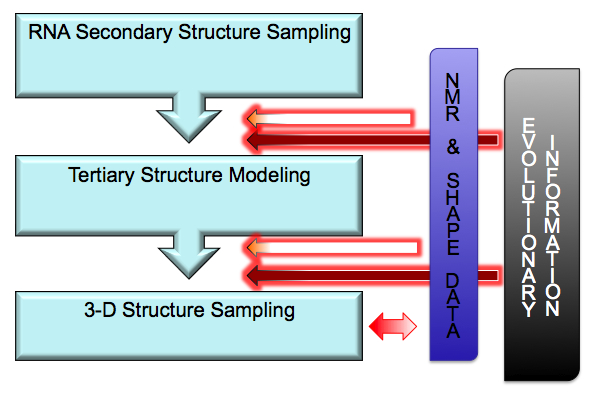
\includegraphics[scale=0.33]{flowchart-pipeline}}
  \subfigure[]{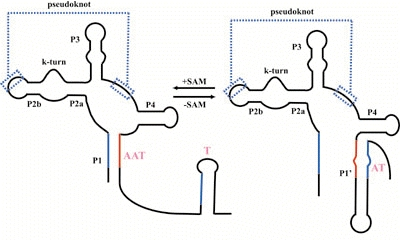
\includegraphics[scale=0.55]{ss-schema}}
\end{center}
\up\up
\caption{(a) The pipeline for riboswitch structure prediction and binding affinity estimation (b) Schematic of the secondary structure change displayed by the SAM-I riboswitch (The left figure represents the OFF state resulted by the SAM-binding and the right figure represents the ON state)}
\label{fig:ribo-pipeline}
\up
\end{figure}

Our current research goals can be understood readily using the pipeline illustrated in Fig.~\ref{fig:ribo-pipeline} and the required computational tasks carried out with the allocation of this request are described below. With the proposed pipeline, we aim to investigate folding dynamics of ribsowtich RNAs and closely related RNA-ligand binding affinity.  This is in contrast to our earlier strategy during which we have heavily relied only upon all-atom Molecular Dynamics simulations.  Indeed, combining multiple computational approaches that differ in their physical principles, increase the chance to achieve a comprehensive understanding of the complex biological process carried out by riboswitch RNAs.  The entire pipeline comprises three steps; the first step represents the Boltzmann Ensemble (BE) sampling of RNA secondary structures, the second step is about the 3D modeling from 2D structure information, and the third step carries out the conformational sampling.  Note that sampling in the first step is executed using RNA secondary structure prediction algorithms, employing the nearest-neighbor energy model and thermodynamics parameters that are experimentally estimated.  The third step is carried out with all-atom MD simulations. The second step represents 3-D molecular modeling using 2-D information.  The requested allocation is primarily support the computational requirements corresponding to the first and the third stages. The BE sampling for the first step is conducted with SFold package\cite{ding2006}.  This type of sampling is typically carried out without the abilitiy to concurrently run multiple simulations, but recently, thanks to the development of a novel runtime environment, we have demonstrated the ``parallel sampling'' of RNA secondary structures using scalable HPC resources (See "Emerging Computational Methodologies in Life Science"~\cite{ecmls10}). For all-atom MD simulations, protocols similar to previous years will be used as described below. As a matter of fact, our pipeline represents the energy landscape perspective that interprets the folding dynamics of a RNA with statistical treatment of an ensemble of structures distributed in the pertinent energy landscape~\cite{onuchic1997}, which has been successfully applied for protein folding but not fully applied for RNA folding\cite{cupal1997}. In our pipeline, the entire folding configuration space is efficiently explored by RNA secondary structure sampling and successively atomistic MD simulations explore the relevant basins of attraction starting from the configurations sampled.

While our pipeline can serve as a de-novo tool for RNA structure prediction from a sequence, it can also be used as a tool box that is able to carry out different physics-based calculations corresponding to each layer, i.e., RNA secondary structure prediction, 3D modeling, and all atom MD simulations for different scientific aims.  This is related to the fact that the nature of RNA folding occurs in a hierarchical manner, implying that the first and the third steps can deal with its own biophysical problems but later findings can be combined for an integrated perspective. Furthermore, our framework uses various computational approaches whose performance relies upon the availability of effective parallel implementation, thus benefiting from TeraGrid/XSEDE like federated, distributed and massively parallel resources.

\begin{figure}
\begin{center}
  \subfigure[]{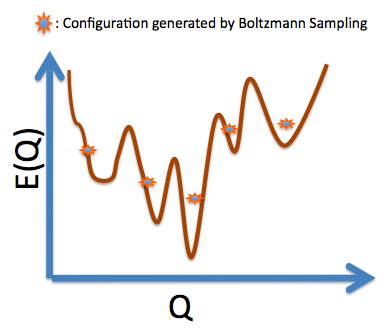
\includegraphics[scale=0.33]{el}}
  \subfigure[]{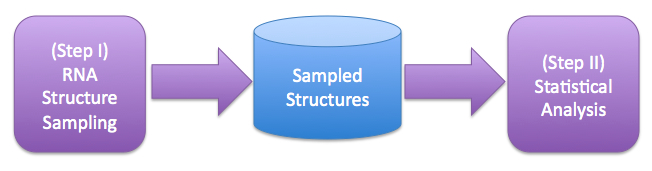
\includegraphics[scale=0.4]{pipeline}}
\end{center}
\up\up
\caption{(a) Illustration of structure sampling in configuration space.  (b) Schematic of a workflow for sampling and analysis of RNA secondary structures obtained with the Boltzmann-weighted sampling}
\label{fig:folding energy landscape}
\end{figure}

A major proportion of our allocation for this project will be used for atomistic MD simulations.  The main goal of the MD simulations is to probe the dynamic interactions between the SAM-I riboswitch and SAM at the nanoscale and to explore determinants for the specificity. In particular, we aim to examine, i) SAM-I riboswitches and their different constructs that differ from each other in potentially different secondary structures and tertiary interactions, ii) different sequences in SAM-I family, and iii) other SAM riboswiches (SAM-II and SAM-III) for which X-ray structures were recently reported and TPP ribosiwtches that we recently started to investigate.  To estimate binding affinity, we employed the Molecular Mechanics - Poisson Boltzmann Surface Area (MM-PBSA) approach using configuration from MD simulations.  As for efficient sampling of conformational dynamics, replica exchange molecular dynamics (REMD) protocol will be used.  REMD calculations will be carried out using available scripts or with our recent development for the distributed adaptive REMD.  

The protocols to be employed are similar to previous protocols.  We will start with a structure derived from the X-ray crystal structures of the AAT conformation of SAM-I riboswitch (PDB: 2GIS, 3GX2, 3GX3, 3GX5, 3GX6, 3GX7)~\cite{montange} or configurations generated by a process via two layers of the pipeline. For a free state riboswitch, SAM is directly removed from the x-ray crystal structure and replaced with solvent water. The amber99bsc0 correction force field is used here~\cite{alberto}. Parameters for SAM are from the Generalized Amber Force Field (GAFF) and missing parameters are calculated using ANTECHAMBER~\cite{wang}. Positions of added hydrogens are guessed using PSFGEN within NAMD 2.6. Then the RNA molecules are solvated in a cubic solvent box of TIP3P waters with a 1.6 nm padding in all directions. Sodium and magnesium ions are distributed around the RNA molecules and neutralize charge of the system. The total number of atoms in the system is 56,000. Energy minimizations are carried out to remove bad contacts. Starting from 0 K, the temperature is raised 10 K every 10,000 steps, and is held constant after reaching the desired temperature (310 K) using temperature reassignment. MD simulations are performed in the NPT ensemble with the pressure maintained using the Langevin piston method with a period of 100 fs and decay times of 50 fs. The time step is 2fs for both equilibration and production phase. Bond lengths between hydrogens and heavy atoms are constrained using SHAKE. The long-range electrostatics is treated with the Particle Mesh Ewald (PME) method with a cutoff distance 1.2 nm.  We use NAMD 2.6.


\begin{figure}%{r}{0.4\textwidth}
\begin{center}
  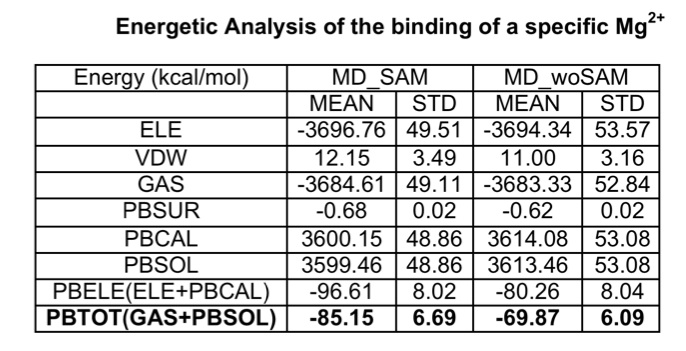
\includegraphics[scale=0.4]{mm-pbsa-mg}
   \caption{MM-PBSA estimation on ${Mg^{2+}}$ binding with a SAM-I riboswitch RNA}
\up\up
\label{fig:mm-pbsa-mg-table}
\end{center}
\end{figure}

Obtained trajectories will be analyzed with various statistical techniques.  Generally, beyond straightforward trajectory analysis measuring various structural variables, PCA analysis and clustering are useful to extract characteristic dynamical motions in terms of reduced dimension techniques\cite{kimjpcb2010, SAM-I-NAR2009}.   Also, we consider the calculations utilizing the Inherent Structure formalism that might reveal intriguing information with respect to the energy landscape properties such as basins, minima, and saddles\cite{kimpre2002,kimjcp2004}.  Conformational dynamics from obtained trajectories of a complex with a ligand and free state will be used for the MM-PBSA calculation with which ligand binding affinity of the metabolites, SAM, or TPP or other related ligands and also for cation binding of ${Mg^{2+}}$ is estimated.  In particular, ${Mg^{2+}}$ binding has been evidenced as crucial for function of catalytic RNAs but remains as elusive for detailed roles in folding dynamics of riboswitches.  Our preliminary results for cation binding are presented in Fig~\ref{fig:mm-pbsa-mg-table}.  According to our preliminary results, this protocol is useful for ranking ligands that bind a pertinent riboswitch, but also we observed that the accuracy depends on the way for entropy calculation and the use of configurations from MD trajectories.  Also, more challenging questions relevant to the validity of force fields that ignores the polarizability as well as the charge transfer effect should be investigated and we hope our calculations provide interesting clues for the answer.      

Sampling the Boltzmann ensemble of RNA secondary structures is the primary strategy to explore the energy landscape efficiently.  We use the SFold pacakge\cite{ding2006} for sampling. The sampling of structures with an input sequence of riboswitches is not computationally intensive, but a considerable number of tasks are required depending on the biological questions.  For example, we carry out comparative investigation on all riboswitches of the same family identified in RFam database; at the moment 2092 SAM-I riboswitches are identified, and the number grows as more genomes are added.  Also, after a sampling step, the analyses involve multi-stage heterogeneous tasks (see Fig.~\ref{fig:folding energy landscape}(b)).  


\begin{figure}%{r}{0.4\textwidth}
\begin{center}
  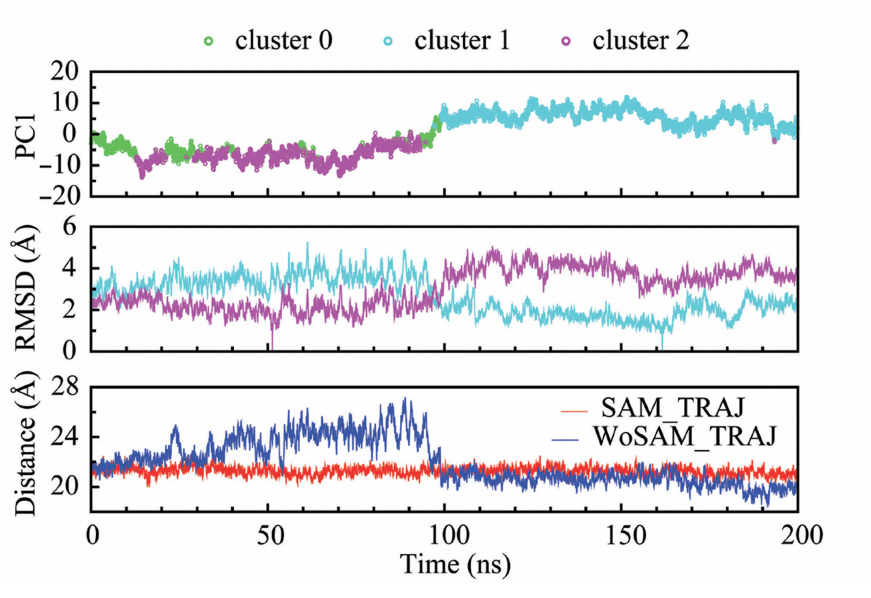
\includegraphics[scale=0.4]{Figure3}
   \caption{ Figure reproduced from~\cite{SAM-I-NAR2009}. The root mean square distance and energetics fluctuate well into the 100-200 ns range. In future simulations, 200ns is a lower bound and we need to go to much longer: at least 300ns.
}
\up\up
\label{fig:Fig3}
\end{center}
\end{figure}


We plan to simulate SAM-I aptamer RNA. Previous time-step benchmarks on Ranger indicate a computation rate of 1ns/82 hours for this 56K atom system on 32 cores. In other words for a 56K system, 1 ns simulations require $\approx$ 300 CPU hours.  Thus each 200 ns simulation requires approximately 60,000 CPU hrs.  Analysis~\cite{SAM-I-NAR2009} results indicate that more than 300 ns trajectory is desirable for observing meaningful conformational dynamics. As figure ~\ref{fig:Fig3} shows, the RMSD of a system starts to stabilize very late in time. Therefore, without additional post-analysis including MM-PBSA calculations, a rough estimation suggest that we can obtain about 100 simulations of a similar system with 1.8M SUs (See {\url{http://staging.teragrid.org/userinfo/aus/namd_benchmark.php}} Boltzmann Ensemble sampling. We are therefore requesting 1.2M SUs on Kraken and 0.8M SUs on Ranger. The small allocation on ranger will be used in the transition phase while we move the rest of the code infrastructure from ranger to Kraken. If the migration from Ranger to Kraken is finished before the allocation on ranger is used up, we will transfer the allocation from the oversubscribed machine (Ranger) to the high availability machine (Kraken). Table~\ref{table:project1} shows the SU request
breakdown for this project.

\begin{table}[!h]
\begin{center}
\begin{tabular}{|c|c| }
\hline 
Resource & Total SUs Requested \\ 
\hline
%1 & Ranger  & TBD \\
Kraken   & 1.2 million SUs \\
\hline
Ranger   & 0.8 million SUs \\
\hline
\end{tabular}
\end{center}
  \caption{SU request for Project 1}\label{table:project1}
\up
\end{table}



\section{Project 2: Atomistic Simulations of Physiological Systems}

The long term scientific objective of our project is to develop molecular dynamics simulations of 
medically relevant enzymes into a tool for clinicians to use in determining the cocktail of drugs to 
administer to an HIV-infected individual. This work is supported by grants under EU FP7 and FP6 
via the VPH-NOE (EU FP7-ICT-2007-5.3 223920), Contra Cancrum (EU FP7-ICT-2007-5.3 223979), 
p-Medicine (EU FP7-ICT-2009-6 270089) and CHAIN (EU FP7 HEALTH-2007-2.3.2-7) projects. For such 
applications, reproducible accuracy at the level which can rank drug efficacies, and rapidity 
of acquisition of results (for clinical relevance) are all essential. This takes the application 
of bio-MD techniques into an entirely new domain. This project is divided into two distinct sub--projects:
(i) Patient specific HIV therapy and (ii) Predicting the affinity of the EGFR kinase domain for drug inhibitors of lung cancer.

\subsection{Subproject 1: Towards Patient Specific HIV Therapy}

\subsubsection{Subproject Progress}
The long term scientific objective of our project is to develop molecular dynamics simulations of HIV-1 Pol enzymes into a tool for clinicians to use in determining the cocktail of drugs to administer to an HIV infected individual. We have recently completed a study which applies our free energy calculation protocol~\cite{Ref2} to a patient derived HIV-1 protease (PR) sequence and the drug lopinavir, identified as producing ambiguous resistance rankings from currently used clinical decision support tools~\cite{Ref3}. This study has suggested a potential new mechanism for drug resistance. We have completed studies of the protonation state of the protease catalytic dyad when bound to all FDA approved HIV-1 PR inhibitors. This is a prerequisite for the application of our protocol to these drugs. With a further allocation we would look to extend this work to compare wildtype and known resistant mutants for each drug.

We have also extended our protocol to investigate the binding of drugs to HIV-1 RT. In this system we have identified the impact of large scale protein motions, distant from the binding site, on the binding free energy~\cite{Ref4}.


\subsubsection{The Case for Continuity}

%%% Yaakoub needs to fix the refs here and shantenu needs to add more capabilities if there
%%% are any
The aim of this project is to calculate binding affinities for HIV-1 enzymes with the anti-viral 
drugs used to target them in clinical practice. We have previously shown an excellent ability to
reproduce experimental results for genetic variants of the HIV-1 protease binding the drug 
lopinavir using ensembles of 50 replica simulations of 4 ns trajectory duration \cite{Sadiq2010}. 
Our work during the current grant has focussed on extending the use of the simulation and analysis 
protocol we have developed to the other FDA approved protease inhibitors (PIs -all of the inhibitors 
included in the study are listed in Table \ref{tab:inhibitors}). 
The initial stage of this process is to access the protonation state of the catalytic dyad of the 
protease bound to each of the inhibitors, which has now been achieved for all drugs. We will be
using the same submission environment: DARE~\cite{dare-tg11} for this project, along with a variety
of community code we have developed from the original allocation (TG-MCB090174).

Having completed our investigation 
of the protonation state used for each inhibitor we performed production binding affinity calculations 
for all of the drugs. Our results produced a promising inter-drug ranking but 
suggested that binding affinities are highly dependent on the initial conformation as well as protonation 
state of the catalytic dyad. It was also observed that results for the inhibitor ritonavir were acutely 
sensitive to the conformation of the aspartic acid at position 30. These observations provide the 
motivation for the future work we will describe in Section \ref{se:hiv_future}.

\begin{table}
\begin{center}
\begin{tabular}{l l}
\textbf{Inhibitor Code} & \textbf{Inhibitor Name}\\
\hline
APV & amprenavir\\
IDV & indinavir\\
LPV & lopinavir\\
NFV & nelfinavir\\
RTV & ritonavir\\
SQV & saquinavir\\
AZV & atazanavir \\
TPV & tipranavir \\
\hline
\end{tabular}
\end{center}
\caption{Code and full names of the HIV-1 protease inhibitors (PIs) investigated.}
\label{tab:inhibitors}
\end{table}

In addition to this progress on the originally proposed simulations, we also extended our previous work 
evaluating the binding affinity of HIV-1 protease mutants to the inhibitor lopinavir. As part of 
a previous collaboration in the EU Virolab project (EU FP7 223131) a comparative drug ranking 
methodology was used to compare drug resistance rankings produced by the Stanford HIVdb, ANRS 
and RegaDB clinical decision support systems. The methodology was used to identify a patient 
sequence for which the three rival online tools produced differing resistance rankings. This process 
identified mutations at only three positions (L10I, A71IV and L90M) which influenced the resistance 
level assigned to the sequence. We have simulated not only the full patient sequences but also 
systems containing the constituent mutations (a total of 12 sequence variants were simulated). 
Inserting any combination of the identified mutations into the wildtype sequence produced no impact 
on the binding affinity of the protease for lopinavir. In contrast when the mutations were inserted 
into the background sequence present in the patient derived sequence resistance was observed. Our 
simulations also identified changes in the relative conformation of the two beta sheets that form 
the protease dimer interface which suggest an explanation of the relative frequency of different 
amino acids observed in patients at residue 71. This study has been submitted for publication~\cite{Owain2011}.

Simulations of the HIV-1 reverse transcriptase bound to the inhibitor efavirenz (EFZ) have also 
been performed. The use of an ensemble approach has revealed that previous single trajectory results 
which allowed the discrimination of wildtype, K103N and L100I/K103N were fortuitous. Consequently we 
performed simulations of only the wildtype, K103N, L100I and L100I/K103N sequences rather than the 
more extensive range of variants proposed. Our results suggest that we need to adapt our protocol here 
to both include more replicas and perhaps to simulate the apo enzyme as well as the drug bound form. 
Simulating the apo form should allow us to evaluate the energetic cost of binding pocket formation 
for each sequence. Simulation conducted as part of this study have shown that experimental differences 
in binding affinity between EFZ and another drug (nevirapine, NVP) can consistently be reproduced.

The resource usage of this project to date is shown in Table \ref{t:hiv_used}. The three studies 
described above are listed as the PR Multiple Drug Resistance Study, PR Virtual Patient Simulations 
and RT Drug Resistance Study respectively.

\begin{table}[h]

\centering
\begin{tabular}[b]
{|c|c|c|c|c|c|}
\hline
\textbf{Sim Description} & \textbf{No. Sims} & \textbf{No. Cores} & \textbf{Code} & \textbf{TG machine} & \textbf{Total SUs}\\
\hline
\multicolumn{6}{|c|}{\textbf{PR Multiple Drug Resistance Study}}\\
\hline
PIs - 6 wildtype PR systems & 380 & 64/48 & NAMD & Ranger/Kraken & 437,760 \\
\hline
\multicolumn{6}{|c|}{\textbf{PR Virtual Patient Simulations}}\\
\hline
LPV - 6 PR sequences & 600 & 64/48 & NAMD & Ranger/Kraken & 345,600 \\
\hline
\multicolumn{6}{|c|}{\textbf{RT Drug Resistance Study}}\\
\hline
EFZ - 3 RT sequences & 30 & 192 & NAMD & Ranger & 600,000\\
\hline
\multicolumn{6}{|c|}{\textbf{PR Catalytic Asp Study}}\\
\hline
7 PIs - WT PR & 240 & 64 & NAMD & Ranger & 276,480 \\
\hline
\multicolumn{6}{|c|}{\textbf{PR Multiple Drug Resistance Study}}\\
\hline
7 PIs - 5 MDR systems & 1750 & 64/48 & NAMD & Ranger/Kraken & 2,016,000 \\
\hline
\multicolumn{6}{|c|}{\textbf{RT Drug Resistance Study}}\\
\hline
Apo RT Wildtype & 10 & 192  & NAMD & Kraken & 768,000\\
\hline
Apo RT L100I/K103N & 10 & 192 & NAMD & Kraken & 768,000\\
\hline
Grand total of SUs used & & & & & 5,211,840 \\
\hline
\end{tabular} \caption{Simulations performed and associated computational cost.}
\label{t:hiv_used}
\end{table}

\subsubsection{Ongoing and Future Work}\label{se:hiv_future}

The previous work in this study has suggested that our free energy protocol is sensitive to particular 
conformations of the catalytic dyad in monoprotonated systems. The two key conformations that can be 
adopted were named `up' and `down' by Zhang \& Zhang \cite{Zhang} and are illustrated in 
Figure \ref{fig:asp_conf}. In order to obtain a correct binding affinity we must start simulations in 
both configurations. We have found that seven of the FDA approved inhibitors have monoprotonated 
dyads and we now wish to run ensembles intialised in the opposite configurations to those already sampled.
This should allow us to more accurately rank protease sequences. Once we have refined out simulation set up
we plan to study each drug bound to a series of mutant sequences with 5 experimentally determined levels 
of resistance. For the protonation studies we propose to use 20 replica ensembles, for the cross drug comparison
we will use 50 replica ensembles. In all cases individual replicas will consist of 2 ns equilibration and 4 
ns of production simulation.

\begin{figure}
  \begin{center}
    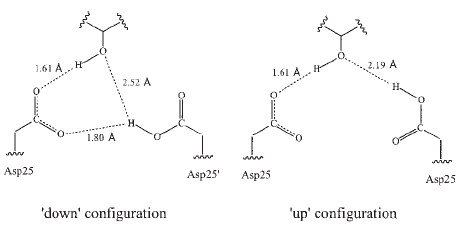
\includegraphics[]{asp_conf}
    \caption{Two conformations of the monoprotonated catalytic aspartic acid dyad of HIV are possible, they are labelled `down' and `up', respectively. The difference between the two lies in the positioning, relative to the ligand of the hydrogen atom. In the `down' position the hydrogen atom is involved in a hydrogen both with the unprotonated Asp25. In the `up' conformation it is involved in a bond with the ligand.}
    \label{fig:asp_conf} 
  \end{center}
\end{figure}

Our reverse transcriptase study indicates the need for simulations of the apo protein we propose to simulate 
10 replica ensembles with 4 ns of production run for the wild type and L100I/K103N double mutant in order to 
replicate the sampling we have achieved for the drug bound systems. 

A further extension of our program of work has involved preliminary studies of the viability of the prototype foamy virus integrase as a model system for investigating resistance in the HIV-1 integrase. This is necessary as no complete structure of the HIV-1 intrasome is available. Our studies indicate that calculated free energies are largely independent of motions of the N terminal domain, which exhibits only low sequence similarity with the HIV homolog, and the DNA substrate~\cite{Ref5}. With further computational resources we would seek to compare the binding thermodynamics of the PFV wildtype with a sequence containing mutations inserted at locations experimentally identified as causing resistance in both PFV and HIV.

Our proposed resource requirements are shown in Table \ref{t:hiv_req}.

\begin{table}[h]
\centering
\begin{tabular}[b]
{|c|c|c|c|c|c|}
\hline
\textbf{Sim Description} & \textbf{No. Sims} &
\textbf{No. Cores} & \textbf{Code} & \textbf{TG machine} & \textbf{Total SUs}\\
\hline
\multicolumn{6}{|c|}{\textbf{PR Catalytic Asp Study}}\\
\hline
7 PIs - WT PR & 240 & 64 & NAMD & Ranger/Kraken & 276,480 \\
\hline
\multicolumn{6}{|c|}{\textbf{PR Multiple Drug Resistance Study}}\\
\hline
7 PIs - 5 MDR systems & 1750 & 64/48 & NAMD & Ranger/Kraken & 2,016,000 \\
\hline
\multicolumn{6}{|c|}{\textbf{RT Drug Resistance Study}}\\
\hline
Apo RT Wildtype & 10 & 192 & NAMD & Kraken & 384,000\\
\hline
Apo RT L100I/K103N & 10 & 192 & NAMD & Kraken & 1,152,000\\
\hline
Grand total of SUs required & & & & & 3,828,480\\
\hline
\end{tabular} \caption{Planned simulations and associated computational requirements.}
\label{t:hiv_req}
\end{table}

We request 4 million SUs: 3.8 million SUs on Kraken and 0.2 million SUs on ranger. The small ranger allocation will be used for transitioning code and and the bulk of the production work will be performed on Kraken. Table~\ref{table:project21} shows the requested allocation breakdown.


\begin{table}[!h]
\begin{center}
\begin{tabular}{|c|c| }
\hline 
Resource & Total SUs Requested \\ 
\hline
%1 & Ranger  & TBD \\
Kraken   & 3.8 million SUs \\
\hline
Ranger   & 0.2 million SUs \\
\hline
\end{tabular}
\end{center}
  \caption{SU request for Project 2}\label{table:project21}
\up
\end{table}


\subsection{Subproject 2: Predicting the affinity of the EGFR kinase domain for drug inhibitors of lung cancer}

\subsubsection{Subproject Progress}
Our research aims at creating molecular level simulators which have an impact in personalized drug treatment of targeted therapy. The epidermal growth factor receptor (EGFR) is a major target for drugs in treating lung carcinoma since it promotes cell growth and tumor progression. Structural studies have demonstrated that EGFR exists in an equilibrium between catalytically active and inactive forms, and dramatic conformational transitions occur during its activation. It is known that EGFR mutations promote such conformational changes which affect its activation and drug efficacy. Using TeraGrid/XSEDE resources, we have been doing two simulations: one is to study changes in drug binding affinities due to cancer mutations of EGFR using ensemble molecular dynamics simulations~\cite{Ref6,Ref7,Ref8}, the other to address activation mechanism of key proteins involved in cancer development and treatment, including EGFR and the GTPase KRAS.

\subsubsection{The Case for Continuity}
We have performed relative binding affinity calculations using multiple (ensemble) short MD 
simulations. Simulations have been run for two tyrosine kinase inhibitors — AEE788 and Gefitinib — 
complexed with wild-type and 4 mutant EGFRs. 50 replicas were used for each molecular systems to 
ensure the calculated properties are reproducible~\cite{Ref6}. In principle, all replicas within a single 
ensemble simulation can easily be run concurrently in one day, thanks to the vast number of cores 
on the XSEDE supercomputers (Ranger for this work). This makes it possible to accurately rank 
drug binding affinities on clinically relevant timescales. We show that ensemble simulations 
correctly rank the binding affinities for these systems: we report the successful ranking of each 
drug binding to a variety of EGFR sequences and of the two drugs binding to a given sequence. The 
study was published recently in J. R. Soc. Interface~\cite{Ref6}.

Long timescale simulations have been performed to study the mechanism of activation by 
cancer-causing mutations within EGFR. Structural studies have demonstrated that EGFR exists in an 
equilibrium between catalytically active and inactive forms, and dramatic conformational 
transitions occur during its activation. It is known that EGFR mutations promote such conformational 
changes that affect its activation and drug efficacy. The most common EGFR mutation in lung cancer 
patients is a leucine to arginine substitution at amino acid 858 (L858R). To investigate the changes 
of conformational equilibrium between the active and inactive states, 4 replicas of EGFR were used 
for each conformation, and 200ns molecular dynamics simulations were performed for each replica. 
Using XSEDE resources, as well as the EU Distributed European Infrastructure for Supercomputing 
Applications (DEISA) allocation, we have performed longer simulations than we initially proposed 
(100ns each). Structural and thermodynamic properties have been extracted from these simulations. 
The thermodynamic stabilities of these two conformations are characterized by free energy landscapes 
estimated from molecular mechanics/Poisson–Boltzmann solvent area calculations. Our study reveals 
that the L856R mutation introduces conformational changes in both states, adjusting the relative 
stabilities of active and inactive conformations and hence the activation of the EGFR kinase~\cite{Ref7}.

The epidermal growth factor receptor (EGFR) is an especially important enzyme target in lung cancer therapy because it mutates and/or is overexpressed in most non-small cell lung carcinoma (NSCLC) tumours. Inhibition of kinase activation of EGFR is a frequently used method to suppress its functions \cite{bib:nature_tki}. The majority of tyrosine kinase inhibitors (TKIs) are ATP-competitive inhibitors which bind in the ATP-binding site. Molecular dynamics (MD) simulations will be used to study the structural and energetic properties of inhibitor-EGFR complexes. The binding affinity of inhibitors to EGFRs will be calculated by molecular mechanics Poisson-Boltzmann surface area (MM/PBSA) methods \cite{bib:wan_philtrans}. This molecular level study is one component of the EU FP7 ContraCancrum (Clinically Oriented Translational Cancer Multilevel Modeling) project which aims at developing a composite multilevel platform for simulating malignant tumor development and pharmacologic responses to a therapeutic intervention (http://www.contracancrum.eu). We have employed large scale MD techniques using both TeraGrid/XSEDE and DEISA resources in order to study the interactions of inhibitors with wild-type and mutant EGFRs \cite{bib:wc2009}.

\subsubsection{Future Work}
A better understanding of the reasons for the success or failure of a therapeutic intervention will help us in the selection of subgroups of patients who are most likely to respond to specific drugs, and paves the way for personalized treatment \cite{bib:hiv}. We have already performed a preliminary study of different inhibitors (AEE788, AFN941 and gefitinib) with EGFR which we now intend to extend to look at a wider variety of inhibitors and EGFR mutations and to probe longer time scale motions of the protein. Planned simulations include ensembles of 50, 50,000 atoms with 25 runs each. Each simulation lasts for 4ns and runs for 9 hours on 128 cores. We therefore request 0.8 million SUs on Kraken to finish this project. The ensemble size and number of runs are typical of established studies~\cite{bib:wan_philtrans,bib:wc2009} of NSF funded research.

We are performing extended timescale molecular dynamics simulations to study the structural and energetic properties of KRAS at both active and inactive conformations. Although studies have provided insights into the structural basis for KRAS activation, the energetic aspects of the conformational changes are not fully understood. We have completed about 250ns simulations so far for wild-type and mutant KRAS within both active and inactive states. To investigate the changes of conformational equilibrium between the two conformational states, substantially longer timescale molecular dynamics simulations are needed. We plan to extend the simulations to ~500ns each. The study will be able to reveal the relative stabilities of active and inactive conformations and hence the KRAS activation. We estimate an additional 0.2 million SUs will be required for these simulations.

We are therefore requesting 1.1 million SUs to continue this project. The bulk of the production simulations will be run on Kraken (1.0 million SUs) and a small 0.1 million SUs allocation is required on ranger to transition the code. The SU request breakdown is show in table~\ref{table:project22}.

\begin{table}[!h]
\begin{center}
\begin{tabular}{|c|c| }
\hline 
Resource & Total SUs Requested \\ 
\hline
%1 & Ranger  & TBD \\
Kraken   & 1.0 million SUs \\
\hline
Ranger   & 0.1 million SUs \\
\hline
\end{tabular}
\end{center}
  \caption{SU request for Project 2}\label{table:project22}
\up
\end{table}




\section{Project 3: Enhanced folding of large RNA ribozymes using Replica Exchange Molecular Dynamics}

\subsection{Project Progress}

We have shown that RNA folds much more rapidly on clay than in a bulk aqueous environment,
but in complex oligomers such as RNA molecules, with many degrees of conformational freedom, folding of the molecule into functional tertiary structures happens over relatively long timescales, which are greater than a typical molecular dynamics simulation (10-100ns). Replica exchange molecular dynamics (REMD) overcomes this limitation through the use of multiple molecular dynamics simulations (replicas) in parallel at multiple temperatures. High-temperature replicas enable rapid barrier crossing and sample additional configurations, which are unlikely to be observed in conventional room temperature molecular dynamics simulations. Periodically, replicas attempt to exchange temperatures according to a Metropolis-like criterion, thereby allowing low-energy configurations to be sampled. Results of our earlier simulations have motivated experimental research in the folding of RNA/DNA on clay minerals at the University of Edinburgh

\subsection{Ongoing and Future Work}
We are currently utilizing TeraGrid/XSEDE resources to progress simulations, which build on our previous publications in the biomaterials domain. Previous simulations performed on TeraGrid resources elucidated the mechanism for adsorption of RNA on montmorillonite surfaces and showed the increased rate of RNA folding into biologically important secondary structures~\cite{Ref9}. Our current simulations have been developed to observe the effects of the clay mineral surface charge on the adsorption and folding of the RNA oligomers. We are simulating large layered double hydroxide (LDH) surfaces with single-stranded RNA molecules of differing sequences~\cite{Ref10}. These large ensembles of models consist of hundreds of thousands of atoms that we hope to progress beyond the standard simulation times of current bioinorganic MD simulations.

Layered nanomaterials consist of mineral layers, such as montmorillonite clays, separated by polymeric or organic material, the thickness of which is of the order of nanometres. The mechanism by which water and other small molecules penetrates (intercalates) between the clay sheets is unknown. To estimate the free energy of intercalation and elucidate the mechanism, we used thermodynamic integration methods. To speed up these expensive simulations, we used multiple replicas of the system at different values of the umbrella constraint and run concurrently using the MD code LAMMPS. 

We propose to use the enhanced sampling available through REMD to explore the conformations of the hammerhead ribozyme absorbed on montmorillonite clay surface. Despite the computationally intensive nature of REMD, it will allow us to determine the role the clay surface plays in mediating hammerhead RNA folding into the most catalytically active tertiary structure. Such a scenario would not be possible with conventional molecular dynamics.

However, in order to get the temperature overlap correct, we will use a reduced model -- a hairpin loop (approximately 10,000 atoms as opposed to the full hammerhead RNA (50,000 atoms).  We have used between 16-32 replicas for the reduced structure per simulation. % Each simulation has roughly 5-10,000 atoms and runs on 32 cores.
A publication detailing these results is currently in preparation~\cite{Ref11}.

Cyberinfrastructure and algorithmic advances in made in the recent \$1.6M Cyber-enabled Discovery and Innovation award (co-PI Jha) will enable the usage of advanced methods to both increase the number of replicas that can be simulated as well as the efficiency of performaing exchanges.



For this project we will estimate we will need a relatively small allocation, 0.4 million SUs on Kraken and 0.1 million SUs on Ranger. This small allocation will be used with in conjunction with the allocation from project 4 (Community Code Development) to run distributed ensembles of REMD simulations on Kraken, Ranger, Lonestar, Blacklight and Trestles. Table~\ref{table:project3} shows the breakdown of requested SUs for this project.


\begin{table}[!h]
\begin{center}
\begin{tabular}{|c|c| }
\hline 
Resource & Total SUs Requested \\ 
\hline
%1 & Ranger  & TBD \\
Kraken   & 0.4 million SUs \\
\hline
Ranger   & 0.1 million SUs \\
\hline
\end{tabular}
\end{center}
  \caption{SU request for Project 3}\label{table:project3}
\up
\end{table}



\section{Project 4: Standards-based Interoperable, Extensible and Scalable Cyberinfrastructure for XSEDE}
In conjunction with the scientific questions we are addressing, we are also involved in the development of a distributed runtime execution system (DARE) that uses the Simple API for Grid Applications (SAGA: http://saga.cct.lsu.edu/)
and higher-level abstractions such as the SAGA-based Pilot-Job (BigJob).

DARE forms the basis of an entire class of Gateways that effectively utilize XSEDE, OSG, LONI and EGI (European Grid Resources) resources. See \url{http://dare.cct.lsu.edu}, for a range of application types.

SAGA-BigJob -- an interoperable Pilot-Jobhas allowed us to run and coordinate hundreds, if not thousands of large-scale ensembles across resources, both on XSEDE and the EU DEISA network, as part of the NSF-HPCOPS funded Interoperability Project~\cite{tg-vph-interop}.  

Significant progress has recently been achieved in enabling the use of SAGA and SAGA-based DARE capabilities to interoperate between different resources -- whether they be different resources on XSEDE or two different grids.  A key goal of an extended allocation would be to further develop the standards-based cyberinfrastructure for XSEDE and assess performance using real scientific workloads, and make it available for the broader \& larger community of biomolecular simulators.

To continue infrastructure development, a small allocation on a number of machines is required. We would like to include as wide an array of different machines as possible to ensure that the infrastructure is portable and easy to deploy. This is particularly important since a large number of the user community (e.g. TG-MCB100145) use different resources. For this reason, we are requesting 300K SUs
 on Lonestar and 100K SUs on both Blacklight and Trestles~\ref{table:Infrastructure}.

\begin{table}[!h]
\begin{center}
\begin{tabular}{|c| c | }
\hline 
Resource & Requested SUs\\ 
\hline
%1 & Ranger  & TBD \\
Lonestar  &  300K \\
\hline
Blacklight &  100K \\
\hline
Trestles  &  100K \\
\hline
\end{tabular}
\end{center}
  \caption{\small Resources requested for continued community code development}\label{table:Infrastructure}
\up
\end{table}

These resources will be used to continue development of the DARE science gateway~\cite{dare-tg11} and its interoperability with different submission systems and work environments. We are asking for non-trivial amount of SUs partly because we need to perform stress tests for scalability testing as well as quality assurance. Running ``/bin/date'' a few times is obviously is not indicative of running hundreds of AMBER/LAMMPS simulations concurrently in a complicated workflow.


\section{Supporting Grants}

The PI's research primary supported by NSF CDI award, CHE-1125332
,``CDI-Type II: Mapping Complex Biomolecular Reactions with Large
Scale Replica ExchangeSimulations on National Production
Cyberinfrastructure'', for \$1.65M for 4 years. The PI's research is
also supported by current NIH and NSF awards.  See PI's vitae for full
grant listing.

Significant work in this proposal is from Work Package 4 of the NSF Funded Cybertools Project (http://www.cybertools.org) -- an NSF EPSCOR Award NSF/LEQSF(2007-10)-CyberRII-01; Total Value \$12M) of which the PI was the lead of the \$2.2M. The PI was till recently the lead of the Computational Biology and Bioinformatics component of the the \$15M NIH award supporting the Louisiana Biomedical Research Network (LBRN) (P20 RR016456-09). % Project 1 is partially supported by the Biosensors work activity of WP-1 of Cybertools.

The first project is funded by multiple awards, including the LBRN Award, Louisiana Board of Regents award and an LSU Faculty Award (PI Jha), in conjunction with multiple awards to Fareed Aboul-ela (Experimental Collaborator). It has also benefitted from a LONI Distinguished Graduate Assistantship to Wei Huang (PhD Student co-supervised by PI Jha and experimental collaborator Aboul-ela). This project forms the basis for a large NSF proposal under review, {\it Macromolecular Choreography: Computational methods to detect conserved dynamic properties in non-coding RNAs}.

The second project is led by co-PI Coveney, who is the Principal Investigator of the \$12M EU FP7 Virtual Physiological Human Network of Excellence. The first two projects are also supported by RealityGrid grant GR/R67699 funded by EPSRC (the UK equivalent of NSF). Coveney and Jha have active collaboration over eight years in the field of molecular dynamics, high performance, distributed \& grid computing and have co-authored over a dozen papers in these areas.
 
PI-Jha is the co-PI of LSU's HPCOPS NSF-OCI 0710874 award which also supports a large fraction of the community code development project. Integration of SAGA with applications is part of Cybertools and the PI also holds multiple peer-reviewed awards for the development and integration of SAGA (EPSRC GR/D0766171/1). %  The Interoperability Project~\cite{interop_url} is currently funded by an NSF HPCOPS award, and is being executed by the PI (Jha).

In addition, PI Jha is the Rutgers-lead in the ExTENCI (OCI-1007115) project that aims to further interoperability between TeraGrid/XSEDE and Open Science Grid.  The community code development project is supported by NSF OCI award - ExTENCI: Extending Science Through Enhanced National Cyberinfrastructure (total \$2M, Rutgers share ~\$0.2M), as well as through NIH grant P20RR016456 and NSF HPCOPS NSF-OCI 0710874 (till March 31, 2012). 


\section{Resource Request Summary}

\begin{table}[!h]
\begin{center}
\begin{tabular}{|c|c|c|c| }
\hline 
Project & SUs on Kraken & SUs on Ranger  & SUs on Lonestar, Blacklight and Trestles\\ 
\hline
%1 & Ranger  & TBD \\
Project 1 & 1.2 million SUs  & 0.8 million SUs & 0 \\
\hline
Project 2 Subproject 1 & 3.8 million SUs   & 0.2 million SUs & 0 \\
\hline
Project 2 Subproject 2 & 1.0 million SUs & 0.1 million SUs & 0\\
\hline
Project 3 & 0.4 million SUs & 0.1 million SUs & 0\\
\hline
Project 4 & 0 & 0 & 0.5 million SUs\\
\hline
\hline
Total  & 6.4 million SUs & 1.2 million SUs & 0.5 million SUs\\
\hline
\end{tabular}
\end{center}
  \caption{Total SUs requested on Kraken and Ranger}\label{table:systems}
\up
\end{table}


The total system time requested for various XSEDE resources is summarized in table~\ref{table:systems}.
We are requesting a total of 6.4 million SUs on Kraken, 1.2 million SUs on Ranger, and 0.3 million SUs on Lonestar, 0.1 million SUs on Blacklight and 0.1 million SUs Trestles. We hope that our utilization track record, large number of publications and community engagement and support will allow us access to the resources we need to continue with our research.


\bibliographystyle{IEEEtran}
\bibliography{saga,Supp,jha_loni_alloc_jul01,ucl_trac,yye00}

\end{document}
